\documentclass{article}


\usepackage{arxiv}

\usepackage[utf8]{inputenc} % allow utf-8 input
\usepackage[T1]{fontenc}    % use 8-bit T1 fonts
\usepackage{hyperref}       % hyperlinks
\usepackage{url}            % simple URL typesetting
\usepackage{booktabs}       % professional-quality tables
\usepackage{amsfonts}       % blackboard math symbols
\usepackage{nicefrac}       % compact symbols for 1/2, etc.
\usepackage{microtype}      % microtypography
\usepackage{lipsum}
\usepackage{wrapfig}
\usepackage{graphicx}

\title{Deep Bayesian Nonparametric Tracking}


\author{
  Rasul Khasianov\\
  Information Science and Technology\\
  SkolTech\\
  Moscow \\
  \texttt{rasul.khasianov@skoltech.ru} \\
  %% examples of more authors
   \And
 Alexander Parubchenko \\
  Data Science\\
  SkolTech\\
  Moscow \\
  \texttt{aleksandr.parubchenko@skoltech.ru} \\}

\begin{document}
\maketitle

\begin{abstract}
Time-series data often exhibit irregular behavior, making them hard to analyze and explain with a simple dynamic model. For example, information in social networks may show change-point-like bursts that then diffuse with smooth dynamics. Powerful models such as deep neural networks learn smooth functions from data, but are not as well-suited in off-the-shelf form for discovering and explaining sparse, discrete and bursty dynamic patterns. Bayesian models can do this well by encoding the appropriate probabilistic assumptions in the model prior. We propose an integration of Bayesian nonparametric methods within deep neural networks for modeling irregular patterns in time-series data. We use Bayesian nonparametrics to model change-point behavior in time, and a deep neural network to model nonlinear latent space dynamics. We compare with a non-deep linear version of the model also proposed here. Empirical evaluations demonstrates improved performance and interpretable results when tracking stock prices.
\end{abstract}


% keywords can be removed
\keywords{Kalman filter \and Variational Autoencoder\and Time series}


\section{Introduction}

The paper focuses on time-series with irregural behaviours. This means that data has sharp bursts. Prices of stocks are one of the possible examples of such time-series. Tracking models like Kalman filter does not suit for task, because bursts can not be modeled. Deep neural nets is also not appropriate for problem, because they fit smooth functions and require additional assumptions to deal with bursts.\\
Thus, authors came up with the idea to connect Bayesian nonparametric methods (further, BNP) and neural nets. The approach is to model time-series through a dynamic change-point model. To do this the authors split time axis into mini-batches. Bursts occur between mini-batches and are modeled by BNP method. Within each mini-batch nonlineraity is modeled by a deep net.

\section{Model}

Basic linear tracking filter is matrix factorization problem $X \approx WH.$ The authors take this idea and develop it. For example, in case of stocks, both matrices are unknown and sequential evolution may be expected in both. Let consider $W$ - a jump process that forms the gloabal structure of data, $H$ - a continuously evolving that models local variations. Then data is represented as $X \approx f(WH),$ where $f$ - neural net.\\
To formilize this let introduce follwing notations: $X \in \mathhb{R}^{I\times N},$ where I - number of items (stocks) and N - number of timestamps.  The authors suggest to split data into T blocks in order to provide the analysis and immitate bursts between blocks. So, the block $X_t \in \mathhb{I \times N_t},$ where $N_t$ - number of timestamps in t-th block. The problem is to find $W_t, H_t$:
$$X_t \approx f(W_tH_t)$$
$W_t$ is assumed to be variance gamma process. Here the partition into blocks helps someone, because he can discretize it. The distribution for each block is 
$$W_t \sim \mathcal{N}(W_{t-1}, \gamma_t I), \gamma_t \sim Gamma(a\triangle s_t, c)$$
The normal distribution means that each row $W_t[i] = W_{t-1}[i] + \mathcal{N}(0, \gamma_t I).$\\
The extension of this approach is to allow for each data stream (each row) to have its own change-points.\\
Matrix $H$ is modeled by discretized Brownian motion:
$$H_{t, j} \sim \mathcal{N}(H_{t, j-1}, \lambda I),$$
where $\lambda$ represents the interval between timestamps. For the first column of block $t$ uses the last column of the previous block.\\
Finally, the authors introduces variational autoencoder framework. They use decoder $p_{\phi}(X_t | W_t, H_t), $ where $\phi$ - decoder parameters, for $t$ block:
$$p_{\phi}(X_t | W_t, H_t) = \mathcal{N}(\mu_{\phi}(W_t H_t), \Sigma_{\phi}(W_t H_t)).$$
This distribution means that each $j$-th column of $t$-th block is under multivariate Gaussian with mean and covariance from a neural net with input $j$-th column of $W_tH_t.$ \\
Moreover, the authors extends the inference of $H_t.$ In VAE approach $H_{t, j}$ is modeled by encoder net, which inputs are $H_{t, j-1}$ and encoded by LSTM $X_{t, j-1}$.
So the distribution on $H_{t, j}$ is:
$$H_{t, j} \sim \mathcal{N}(\mu_{\theta}(S_{t, j-1} H_{t, j-1}), \Sigma_{\theta}(S_{t, j-1} H_{t, j-1})),$$
where $\theta$ - encoder parameters, $S_{t, j-1}$ - hidden state of LSTM for cell with $X_{t, j-1}$ input.


\section{Implementation}
Let's discuss more about implementation of autoencoder. From this paper we have coded encoder to sample posterior $H_t$, decoder.


% \begin{wrapfigure}{l}{0.4\textwidth}
%   \begin{center}
%     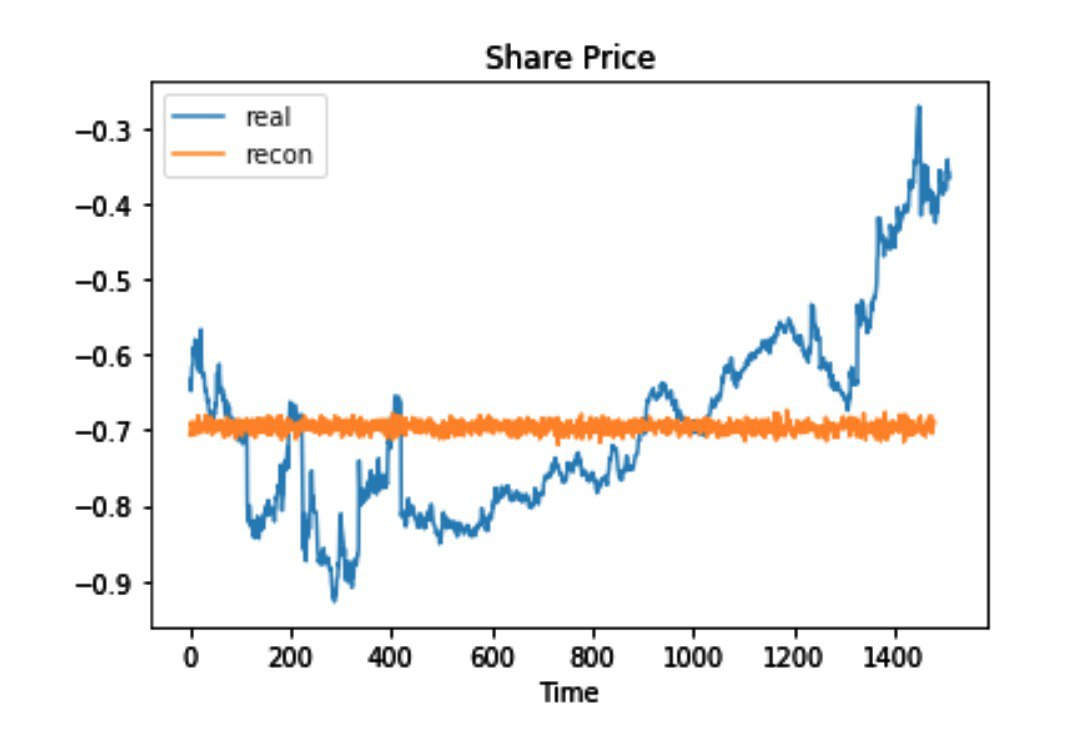
\includegraphics[width=0.4\textwidth]{img1.png}
%   \end{center}
%   \caption{Predictions}
% \end{wrapfigure}

\subsection{Encoder}
To exploit the sequential structure of the data, we use LSTM to encode $X_t$. The output of LSTM $S_t$ we use as hidden layer for feed-forward neural network.


For each $j$ column we concatenate columns $S_{t, j-1}$ and $H_{t, j-1}$ into a single vector $(S_{t, j-1}, H_{t, j-1})$. We feed this vector to two feed-forward neural networks. These neural networks give us parameters of Gaussian distribution $\mu_\theta, \Sigma_\theta$, where $\theta$ -- parameters of neural network. Finally, we can sample new column of matrix $H_{t, j}$ by using reparametrization trick. 

In this step we have $2 N_t$ feed-forward neural networks. 
\begin{figure}[h!]
  \begin{center}
    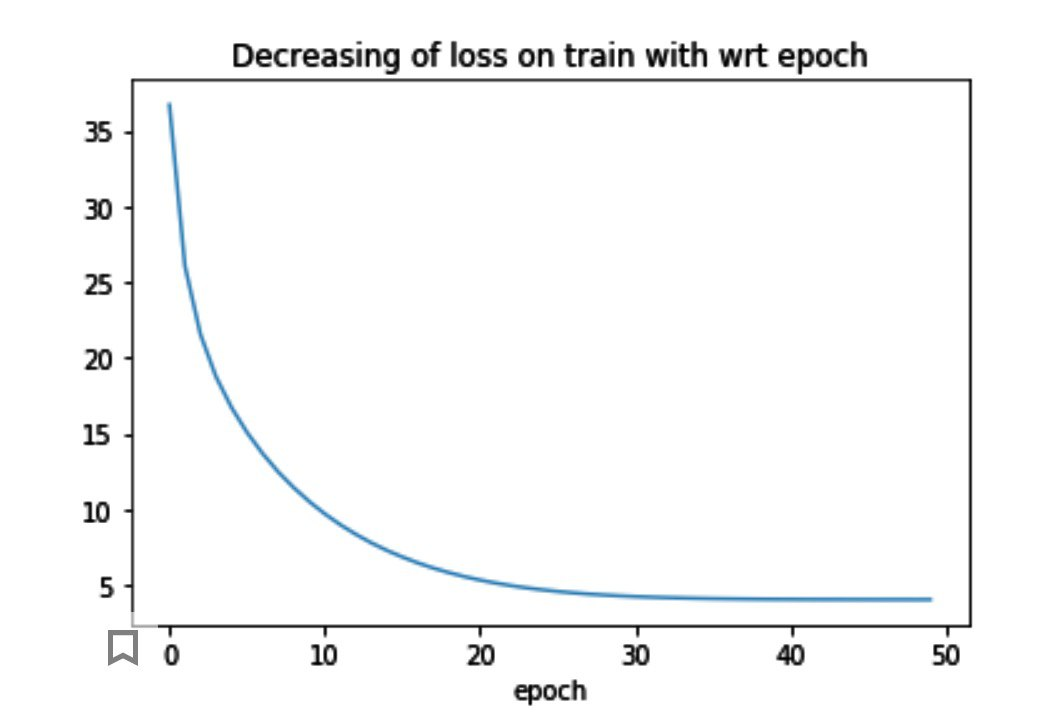
\includegraphics[width=0.4\textwidth]{img.png}
    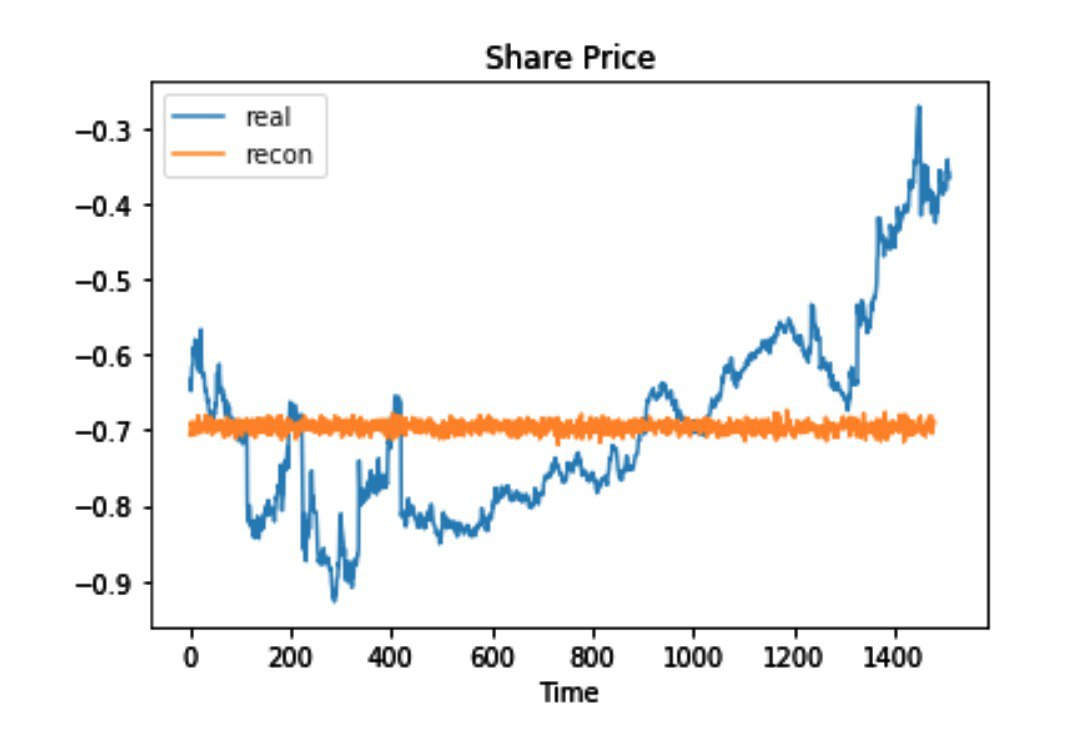
\includegraphics[width=0.4\textwidth]{img1.png}
  \end{center}
\end{figure}

\subsection{Decoder}
Implementation of decoder is very obvious. We just multiply matrix $W$ and column of matrix $H$ and pass it into feed-forward neural netwroks to obtain parameters of Gaussian parameters.
$$p_\phi(X_{t,j} |W, H) = N(\mu_\phi(W_t H_{t,j}), \Sigma_\phi (W_t H_{t,j})$$


\section{Experiments}

We have downloaded data from Quandl from 200 companies. The data from 2008-2012. We have trained model on 50 epoch. Unfortunately, prediction of this model wasn't so good. 


% \subsection{Figures}
% See Figure \ref{fig:fig1}. Here is how you add footnotes. \footnote{Sample of the first footnote.}

% \begin{figure}
%   \centering
%   \fbox{\rule[-.5cm]{4cm}{4cm} \rule[-.5cm]{4cm}{0cm}}
%   \caption{Sample figure caption.}
%   \label{fig:fig1}
% \end{figure}



% \bibliographystyle{unsrt}
% \bibliography{references}

\end{document}
